\documentclass[12pt,a4paper]{article}
\usepackage{fontspec}
\defaultfontfeatures{Mapping=tex-text}
\usepackage{xunicode}
\usepackage{xltxtra}
\setmainfont{FreeSerif}
\setmonofont{FreeMono}
\usepackage{polyglossia}
\setdefaultlanguage{english}
\usepackage{amsmath}
\usepackage{amsfonts}
\usepackage{amssymb}
\usepackage{siunitx}
\usepackage{xcolor}
\usepackage[justification=centering, font={small, sl, color=gray}]{caption}
\usepackage[margin=2.5cm]{geometry}
\usepackage[section]{placeins}
\usepackage{datetime}
\usepackage{hyperref}
\usepackage{indentfirst}
\usepackage{enumitem}

\author{Anas Naïri \and Julien Plante}
\title{Modelisation of ExoMars 2020's network using SystemC}

\setlength{\parindent}{0cm}
\newcommand{\Cpp}{C\texttt{++}}

\begin{document}

\begin{titlepage}


\includegraphics[width = 60mm]{pictures/suai.png}

    \vspace*{\fill}

    \begin{center}
    
        \Huge\bfseries
        Second R\&D project report
        \vskip10pt
        \Large\bfseries
        Modelisation of ExoMars 2020's network using SystemC
        \vskip10pt
        \large
        PLANTE Julien - NAÏRI Anas
        \vskip20pt
        \large
        Saint Petersburg State University of Aerospace Instrumentation.
        \vskip20pt
        
        \vspace*{\fill}
        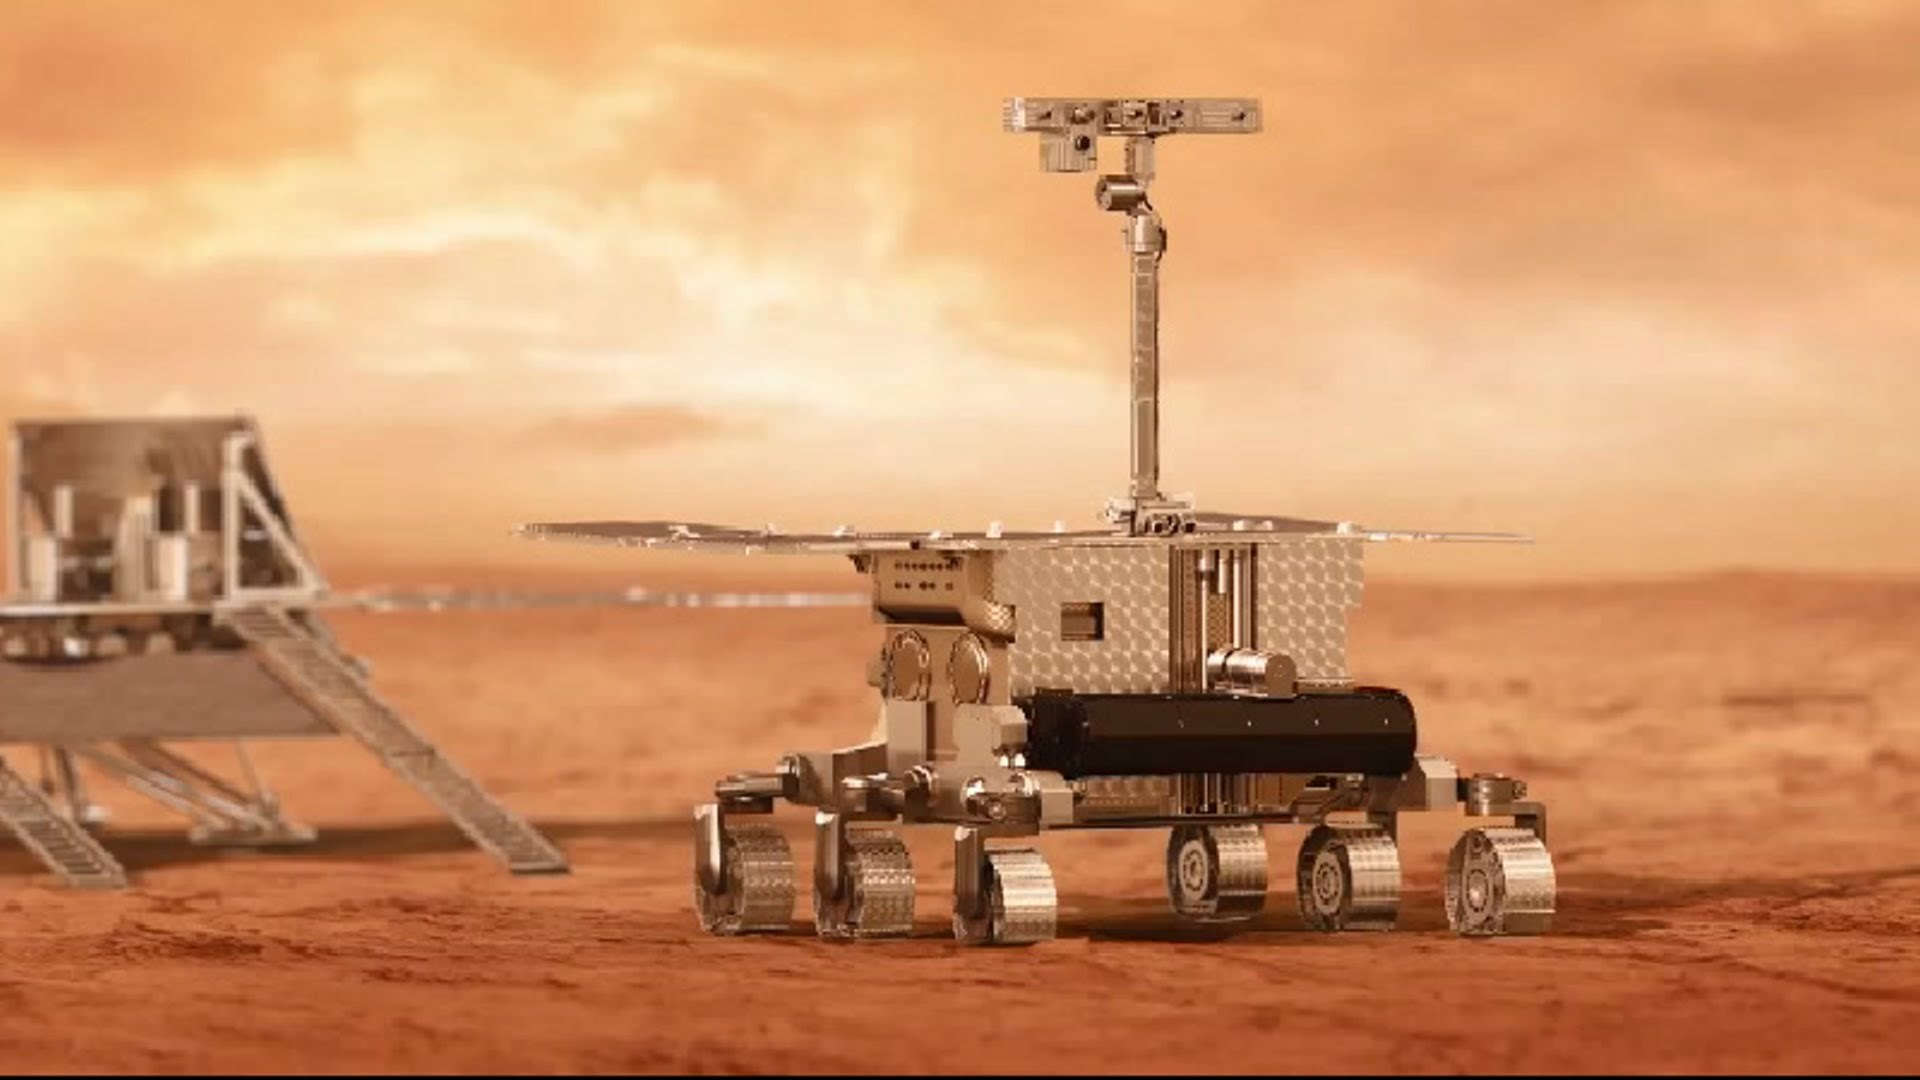
\includegraphics[scale = 0.2]{pictures/Exomars2020.png}
    \end{center}
    
    \vspace*{\fill}

\end{titlepage}

\pagebreak

\tableofcontents

\pagebreak

\section{Task formulation}

\begin{itemize}
    \item Read documentation about the ExoMars2020 rover to establish the rover's network structure
    \item Implement the rover's network on SystemC, only the SpaceWire's network layer. Channels must handle the speed of transmission and error bit frequency, and devices must generate data into the network and receive data from it
    \item Create a base log-system to record results of the simulation through SQlite
    \item Split the network into two different parts to parallelise, and compare the modelling time between a single model and a parallel model
\end{itemize}
\section{Introduction}

Our second project is a direct continuation with the previous one. To summarize briefly, our first R\&D project was about implementing a SpaceWire network using SystemC, to simulate data sent from Earth and received on a spacecraft.\smallbreak

In fact, this R\&D project, which is to simulate the data-handling network architecture of the ExoMars2020 rover, involves to use a SpaceWire router with a view to interconnecting the multiple scientific instruments. Since the rover uses a lot of cameras to observe, analyse and interpret its environment, the processing of images taken by these instruments is well needed. In that case, as we can see in the figure below, the rover got a dedicated chip for this kind of process. Data will be sent from equipment, then to the memory, next to the processor which will give instructions to the image processor.\smallbreak

\begin{figure}[hb]
	\centering
    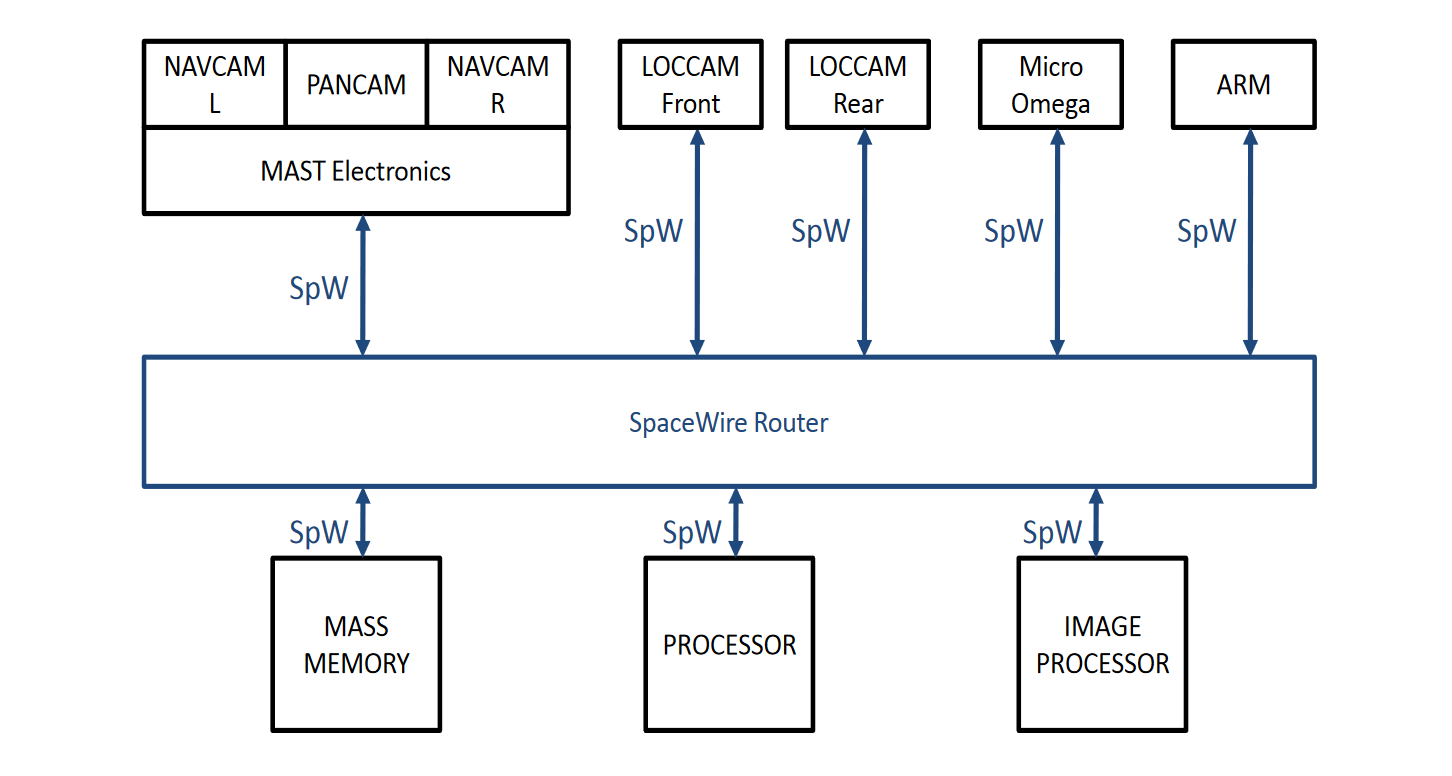
\includegraphics[scale = 0.49]{pictures/data_network_architecture.png}
    \caption{Data-handling structure of ExoMars' rover}
\end{figure}

Consequently, such amount of image transmission can be well handled by the use of a SpaceWire router, because, as we already know, SpaceWire is a good data-handling network which allies high speed of communication, low power consumption, and low cost implementation. It is ideal in the case of ExoMars2020, because it needs to connect all equipment to memory and processors. We also read that the ExoMars2020 rover uses the RMAP protocol to communicate and exchange data between different nodes, and it is an interesting task to implement this protocol, since it gives us a real packet structure, and a more accurate representation of what happens in SpaceWire networks than during our first task.\pagebreak
\section{Description of ExoMars2020 rover}

The ExoMars2020 mission has for goal to search evidence of past or present life on the surface and/or subsurface of Mars. Thanks to its rover, it will, in addition, understand more the planet's surface and subsurface, like its origin of formation and the composition of it, by the use of multiple scientific instrumentation as cameras, radars and spectrometers.\smallbreak

\subsection{PanCam}
The PanCam is used to record 2D \& 3D images of the Mars' surface, in order to understand the geological and morphological situation on the planet. In fact, the PanCam is composed of two WAC (Wide Angle Camera), one on the left, the other on the right to have a stereoscopic view of the ground, and a HRC (High Resolution Camera). Also, it operates to produce images in the near infrared and visible wavelength. This device, in synergy with the others, allows the rover to chose the best potential locations site to drill, for example shallow ground that may contains gases or water. The HRC and WAC, both operates with an image resolution of 1024 x 1024 pixels, the first one in RGB, the second with a multispectral filter wheel. The PanCam communicates with packets of 10-bit data.

\begin{figure}[h]
\centering
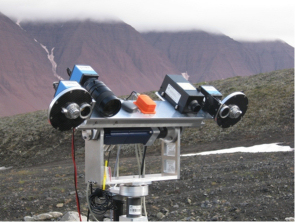
\includegraphics[scale=1]{pictures/PanCam.jpg}
\caption{The PanCam prototype during tests in Mars-like conditions\\Credit: AMASE}
\end{figure}

\subsection{ISEM}

The ISEM (or Infrared Spectrometer of ExoMars), as its name means, is an infrared beam that senses the infrared part of the sun's light reflection onto Mars' surface. With this method used on the rocks near of the rover, it obtains the spectrometer of these rocks and then get information about the geological composition of the planet's surface. Indeed, this device helps the rover to chose a potential location to drill in, because the presence of some minerals may indicate good places where to find past life on Mars. It communicates using packets of 16-bit data.

\subsection{CLUPI}

The CLUPI, or Close-Up Imager, is a high-resolution camera which goal is to take close picture of rocks to be able to detect each details of these ones. Thus, we can know to what type of rock we are seeing or surrounded with, by analysing the texture, the color, the morphology, etc. Also, it will give information about the original context of possible formation of these rocks, like, geological major events that they experienced throughout their existence. Plus, with this kind of close up pictures, we should be able to detect bio-signatures at the surface of rocks. It is permitted because the CLUPI has an image resolution of 2652 x 1768 pixels in RGB. It can take picture in the visible wavelength, with an exposure time of 1024 seconds. It communicate with packets of 14 bits.

\begin{figure}[h]
	\centering
    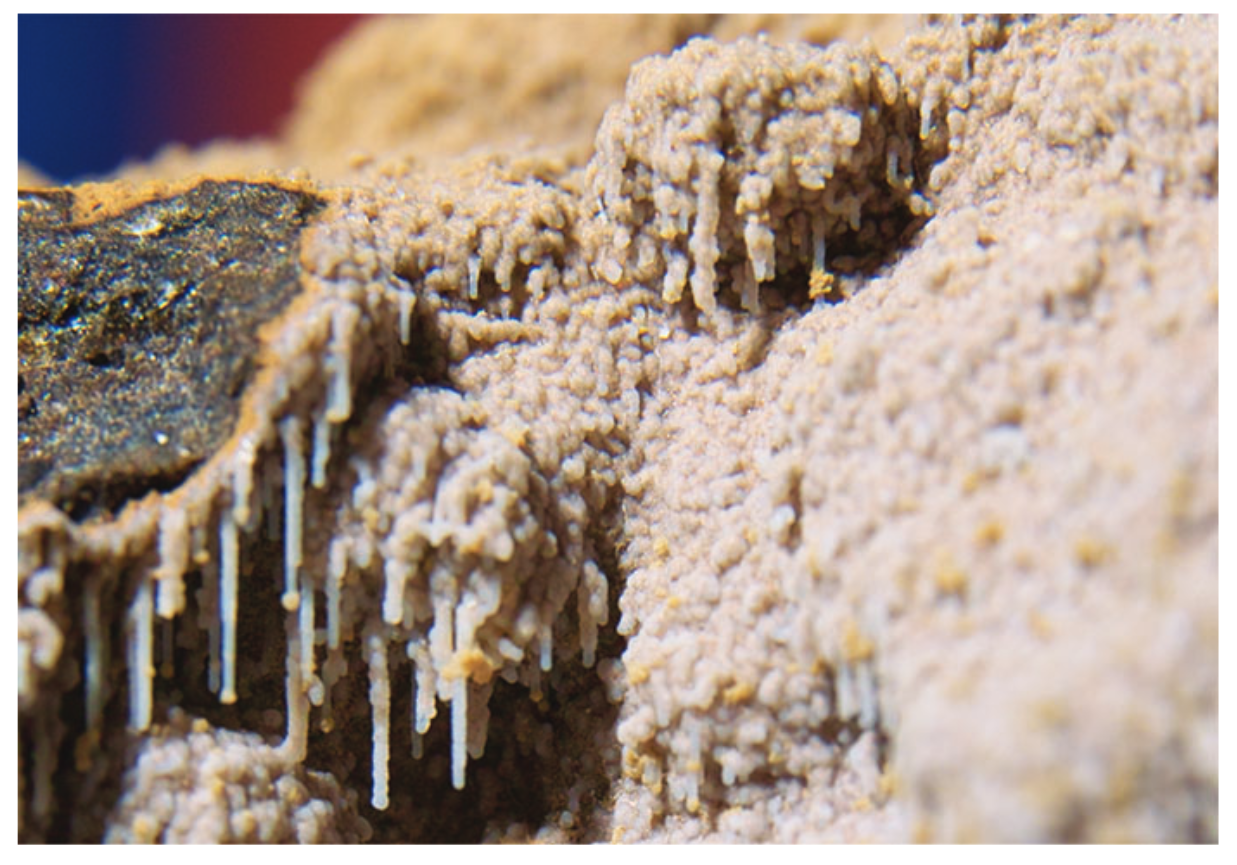
\includegraphics[scale = 0.5]{pictures/close_up_image.png}
    \caption{Close up picture of a rock taken from CLUPI}
\end{figure}
\subsection{WISDOM}

To find if there are some evidence of the past and present life on Mars, we can search in the subsurface, where organics molecules could be shielded from destructive events. In fact, the WISDOM, or Water Ice Subsurface Deposit Observation on Mars, is a ground penetrating radar which will help to notify and describe the type of the shallow surface that is pointed by this one. If an information about a place in subsurface has been processed as a potentially location of organics molecules, the ExoMars' drill will then dig in it.\smallbreak

In addition, WISDOM is working with others instruments to precise if a place in the subsurface is relevant or not by gathering information from Adron, PanCam and Ma\_Miss. From the Adron, we can obtain information about the composition of a source of water in liquid or ice form. From the PanCam, we get 3D information of the rover's environment, that can help it to better filter locations to dig in. And, because the Ma\_Miss is in the drill, it is in direct contact with the subsurface, thus data from this one are compared with those from WISDOM that will permit to set a 3D map of the subsurface. By the way, WISDOM communicate with other equipment by packets of 16-bit data.

\subsection{Adron}

The Adron is a detector of radiations of neutrons that are sensed from the subsurface of the planet. With the data from WISDOM, it permits to detect the water distribution in the Mars' subsurface and the presence of certain elements in this water. Then, the combination of the both instruments' data would help to localize the best places to drill in order to find evidences of potential past or present life on or below the surface of Mars. It communicate with packets of 9-bit data.

\subsection{Ma\_MISS}
Ma\_MISS, for Mars Multispectral Imager for Subsurface Studies, is a spectrometer located in the drill of the rover, used to determine horizontal and vertical composition of the Martian soil. By illuminating the borehole and analysing the reflected light and its spectrum, it will be able to gather information about the distribution of minerals, especially of water-related ones, to search potential indicators of life.

It will work alongside the three other spectrometers (RLS, MicrOmega, MOMA), being specialised in studying unexposed material, and in collaboration with WISDOM and ADRON to choose interesting drilling location

\begin{figure}[h]
\centering
\includegraphics[scale=.7]{pictures/MaMiss}
\caption{The instrument, located on the drill.\\Credit: SELEX Galileo}
\end{figure}

\subsection{MicrOmega}

MicrOmega is an infra-red spectrometer made to identify composition of Martian soil samples at a grain scale, after their gathering by the drilling system. It is similar as RLS and MOMA in this way, since the three spectrometers will study samples collected by the drill. The infra-red study of the samples is adapted to find evidences of past or present carbon and water presence. 
It uses an infra-red hyper-spectral microscopic imager to acquire the spectrum of a 250$\times$256 pixels square (\char`\~5$\times$5 \si{\milli\metre^2}) for 320 wave length, between 0.95 and 3.65 \si{\micro\metre}. Thus having a maximum of \num{20480000} bytes to transmit.

\subsection{RLS}
RLS uses the Raman effect to find life signatures in Martian soil samples in a non-destructive way.
The measurements carried out by the RLS will be performed as described within the ExoMars Rover Reference Surface Mission, which includes six experiment cycles (with two samples each, one extracted from a surface target and the other at depth) and two vertical surveys (with five samples each extracted at different depths). It generates information about a 2048$\times$512 pixels of 15 \si{\micro\metre}, totalling a surface of approximately 30.7$\times$7.7 \si{\micro\metre^2}, and \num{1048576} bytes.

\subsection{MOMA}
MOMA (Mars Organics Molecule Analyser) is an instrument designed to detect organic molecules in spots of interest detected by the collaboration of RLS and MicrOmega, thus providing extremely precise analysis of Martian environment, and great information about potential origin, evolution and distribution of life on the planet. To do so, it will study samples gathered by the drill, as well as analysing the gases of the Martian atmosphere. It features to modes of operation : Gas Chromatograph-Mass Spectrometry (MOMA GC-MS) and Laser Desorption-Mass Spectrometry (MOMA LD-MS), the first one being used to analyse atmosphere gases, and the second soil samples. No information about size of data produced was found.

\begin{figure}[h]
\centering
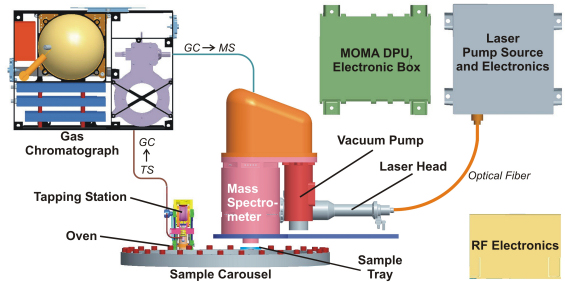
\includegraphics[scale=.7]{pictures/MOMA.jpg}
\caption{The MOMA instrument and its modules.\\Credit: Max Planck Institute for Solar System Research}
\end{figure}

\pagebreak

\section{Model structure and functioning description}
\smallbreak
The final structure of our project looks like this: \smallbreak
\begin{figure}[h]
\centering
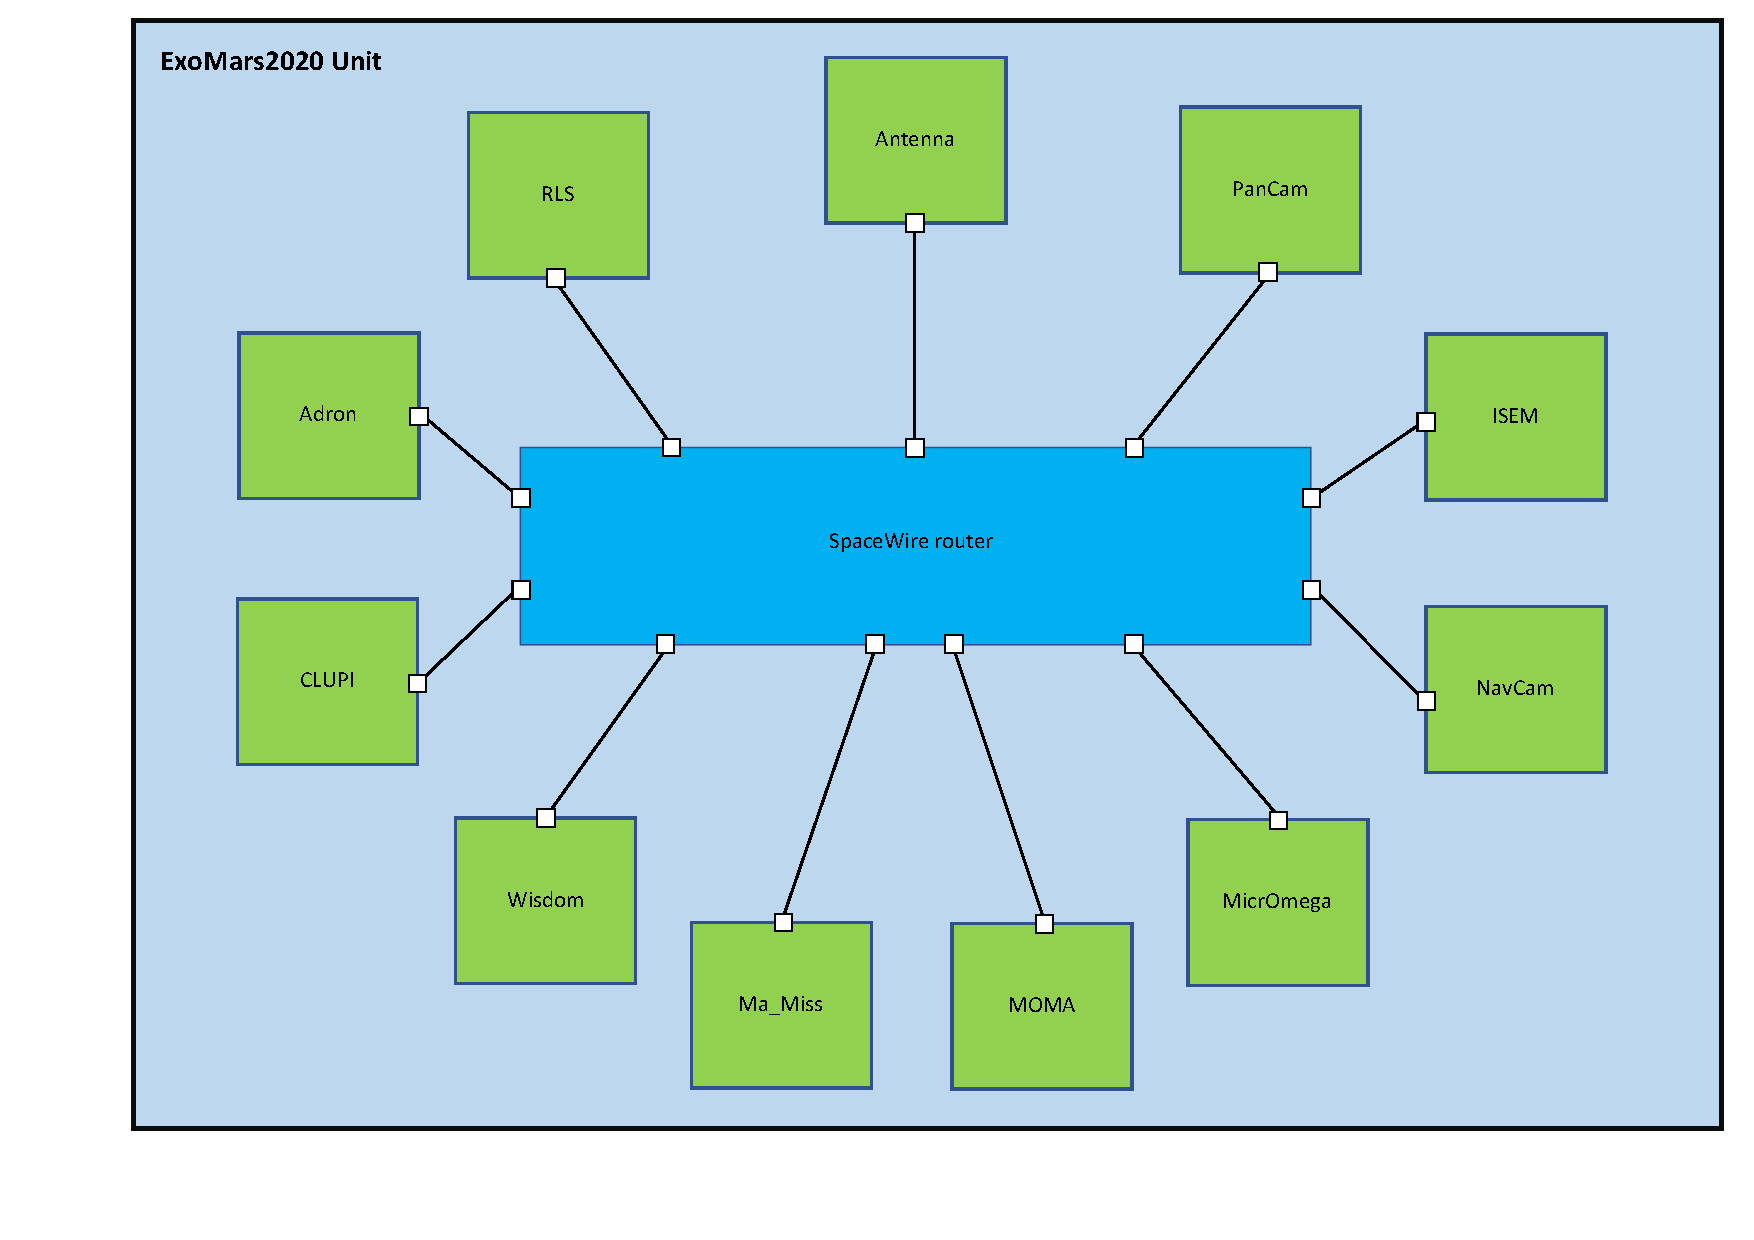
\includegraphics[scale=.5]{pictures/structure_ExoMars2020.pdf}
\caption{Final structure}
\end{figure}
\smallbreak

As in the first task, the SpaceWire Router is modelled by the \Cpp class \texttt{SwitchUnit} and the top module containing all the others by \texttt{NetworkUnit}. But one major difference is that each node is modelled by the same \Cpp class named \texttt{Node}, specialised thanks to a configuration file. This was made in order to avoid boilerplate code, since all nodes have a similar behaviour, errors due to wrong copy of new functionalities in each class, and to prepare the work for a more complex simulator, using a GUI to configure any SpaceWire network.

All details about these improvements will be explained in the following subsections.

\subsection{Features}
\subsubsection*{SpaceWire}
Our project features the modelling of the the third OSI layer of the SpaceWire specification, as requested, but also of a part of the second layer, since it was already done during the first task.

The third OSI layer covers the use of packets to transmit data from one node to another, with possible routing on the way. About the second layer, we modelled only a part of it, since it was kept from the first task and was not mandatory for this one. We only have the transmission by frames of packets, allowing for transmission delay simulations and transmission error modelling (due to some possible incident radiation). It also made us think on the problem of data collision, since we used bidirectional channels, and forced us to create some security mechanism. But we did not implement the Error End of Packet (EEP) and error link recovery at this level.

The only communication protocol implemented is RMAP, since we found out that ExoMars2020 uses this protocol. More details about its implementation can be found in the description of \hyperref[ssec:Node]{Node}
\subsubsection*{Log system}
We added a logging system, to increase debugging possibilities. It was at first under the form of a simple text logging.The information printed to the standard output was also written to files, with one log for each node, resulting in a less mixed output. But this was not very practical, since analysis on these files was tedious, because of no formal format used. This is why we quickly decided to investigate database logging, which was one optional task.

We chose to use SQLite as database, since its use was much simpler and more adapted (at least at the moment) than MongoDB, the other database client investigated. Indeed, we wanted to use database as a handy file format to store our information, which is easily allowed by SQLite, which stores everything in one file. MongoDB on its side uses the client/server paradigm, and would have forced us to go through the localhost, bringing complications. We successfully logged packet transmission using SQLite, and the ability to perform SQL requests proved its interest, allowing us to find bugs, and permitting custom analysis of what happened during the simulation after its end.

\subsubsection*{Parallelisation}
We were asked to separate our network into two different parts, and paralellising the simulation. Indeed, we transmit in the network big packets, and the simulation began longer and longer as we added features. An idea to increase simulation speed was to run the two independent parts of the network in parallel, hoping for a performance increase. To do so, we described the two distinct parts using a configuration file (see below), and used preprocessor directives alongside preprocessor definitions to compile two different executables, each one of them being able to simulate one part of the network. We then used the Windows API, and the function \texttt{CreateProcessA} to run the two parts concurrently.

\subsubsection*{Configuration file}
As already explained, we used a configuration file to describe nodes behaviour and different parts of the network. It is also specifies parameters of the channels, which are the same in the whole network, which could be a limitation, but could also be tweaked.

At first, we used a custom configuration file and wrote the parser ourselves. It was doing the job, but adding functionalities was complicated and error prone, and the parser itself not very fault tolerant and strong when facing syntax mistakes. Moreover, we had the idea of a GUI to describe all the parameters, and judged that it would be harsh to interact with our custom configuration file.

So we moved to the JSON format, using the header-only \Cpp JSON parser RapidJSON. It proved to be much stronger, and allowed us to easily add new features, without needing to check for bugs. It currently supports channels specification, network part specification, nodes declaration, description of their interaction with the network (when to send packets, how many, the type \textsl{etc}), and the self generation of packets, modelling an experiment where results are stored in a node's memory, with similar arguments. The only limitation of this configuration file is that it doesn't allow to describe routers for now, so one router is created for each network part. 

To easily gather information from the DOM, we wrote a loader contained into a class, which can be found in \texttt{helperlib.h} and the corresponding implementation file \texttt{helperlib.cpp}.

\subsubsection*{Graphical User Interface}
Another optional task we began is the Graphical User Interface (GUI). Sadly, we didn't have time to finish it, but is still an interesting feature of the project.

We chose the Qt framework to develop it, since it's one of the most developed widget toolkit with GTK\texttt{+}, and seemed easier to use than the later, since it is written in \Cpp and thus doesn't need bindings, which is the case for GTK\texttt{+}. Moreover, the existence of QtDesigner allowed us to easily design our UI and quickly obtaining interesting results. At the time of writing, it is able to generate the configuration file, compiling and starting simulation of the different parts of the network, and also analysing the results thanks to a simple SQLite database viewer.

Planned improvements are reading from existing configuration file to load network parameters, network part management when editing nodes, and possibility to choose from which database we want to read, as well as a refresh button for the database viewer.
Further possible, but hypothetical improvements could be to add a graphical representation of the network, and a graphical editor, instead of parameters only, and real time animation of the graphical editor during the simulation.

\subsection{Network Unit}
\texttt{NetworkUnit} kept its role since our first task and the corresponding report, namely to instantiate all the others modules and linking them with channels. But its way to do this changed drastically, since everything is allocated dynamically, to allow customisation through the configuration file.

To do so, it firstly recover all the configuration needed using the \texttt{JsonConfigLoader}. It then dynamically allocates every node, which pointers are stored into the vector \texttt{instruments} to keep a handle on each one of them. The same is done with channels. At the same time, we connect the instrument to the channel and the router, using the function \texttt{SwitchUnit::connect} that creates routing tables automatically. 
\begin{quote}
Remark: One of the goals after the first task was to increase memory safety of our application, since we used \texttt{new} and \texttt{delete}, which can cause memory leaks if the deallocation is forgotten or in case of a crash, if stack unwinding doesn't happen. This is why we used \texttt{make\_unique}, and \texttt{std::unique\_ptr<T>} declared in the header \texttt{memory}. This is a smart pointer, deallocating memory when going out of scope, and thus safer than raw pointers.
\end{quote}

After that, \texttt{NetworkUnit} adds other parameters of the config file to the nodes created, concerning generation of packets and transmissions they have to do.

This module is also in charge of opening the database and passing its pointer to each node, as well as creating the trace file and make it watch each channel. Its definition can be found in \texttt{networkunit.h} and the implementation in \texttt{networkunit.cpp}.

\subsection{Node}
\label{ssec:Node}
This module describes a SpaceWire node with only one port, that can be configured to our need through the configuration file. It contains multiple methods, corresponding to multiple levels of abstraction in our model of the node, which were useful to structure the code. They contain a memory that can be written or read through the RMAP protocol, or written directly by the node itself, simulating the generation of data. Since RMAP is a well known standard, we decided not to describe it in this report, but more information can be found in \cite{RMAP}\medbreak

Firstly, there are three type of daemons, which are by the way the three main type of threads of this module (we named them daemons because it usually describe threads that run in the background, handling everything important). The main one is \texttt{receiver\_daemon}, in charge of handling reception of packet, and choosing what should be done with the packet. It is written to receive RMAP packets, and sending back replies if needed. This daemon is only launched once, and runs during the whole simulation, which is not necessarily the case of the others. \texttt{sending\_daemon} and \texttt{generating\_daemon} are very similar, the first one being in charge of sending RMAP commands, and the second one generating data directly to the node memory. Any number of these two can be spawned, according to the fields "Connections" and "Generations" of the config file. They can also terminate before the end of the simulation, if their role is finished.

Secondly, the function \texttt{send} allows to send a packet of any type, and waiting for a reply. If the reply has a positive status (1), the function ends, and if the status is 0, the packet is sent again, until a positive status is received, allowing for safe communication and error recovery. There is no \texttt{recv} function currently, since we only use the reply as acknowledgement packet, but we could create a \texttt{recv} function that sends an acknowledgement back, for both commands and replies.

Finally, the function \texttt{send\_raw} and \texttt{recv\_raw}, at the lowest level, each one having as parameter one packet and which are respectively in charge of sending actual data into the port and receiving actual data, determining the type of packet and accordingly create the correct packet before returning. One interesting difficulty for the \texttt{recv\_raw} function was that RMAP uses different header structures for different actions, and we had to determine the type of the packet one the fly, while receiving, to correctly determine the end of the header, and the beginning of the data.\medbreak

This module also features regular logging and database logging, which are not its first role, but still key points, especially for debugging and analysis of the model. Tables are firstly created in the database, to be ready to store data in the member function \texttt{init\_db}. Packets are after that automatically stored whenever one is sent or received.

The definition of this module can be found in \texttt{Node.h} and the implementation in \texttt{Node.cpp}.

\subsection{Packet}
This class aims to simplify communication throughout the network, and clearly separating layers 2 and 3 of the OSI model. It contains two vectors, one for the header and one for the data, since each part is of variable size in the RMAP protocol, as well as two checksums (CRC), for the header and the data. Data can be inserted or extracted as it would be done for a stream, using operators \verb|<<| and \verb|>>|, which allows to compute the CRC on the fly, as it would be done in a real equipment. But this interface is not always handy, and we needed to add functions about the end of the header, because of the variable header size of the RMAP protocol, and maybe the class would need a rewrite to provide simpler interface.

That being said, it is very useful to contain packets simply, more than the FIFOs we used during the first task, and can be printed in a clean way through the overloading of  \verb|operator<<|.

The definition of this module can be found in \texttt{Packet.h} and the corresponding implementation in \texttt{Packet.cpp}.
\subsection{SwitchUnit}
\texttt{SwitchUnit} didn't change a lot. We just increased memory safety by dropping the bidimensional C-style array we had before for a \texttt{std::vector}. We also added the simple \texttt{connect} function, that allows to connect a node to the router through a channel, and automatically modify the routing table to match the new connection. The only limitation here is that we didn't write any \texttt{connect} function to link two routers, but we didn't need this at the time of writing, since ExoMars2020 contains only one router. But if we are to develop a more complete and versatile simulator, this could become a need.

\pagebreak

\section{Simulation results}

\subsection{Console output}

ANAS

\subsection{Traces}

ANAS

\subsection{Modelling time comparison}

ANAS

The ExoMars2020 in our project is composed of many several equipment, which are divided into two main parts : the mast and the main body of the rover. The mast can be composed of the PanCam, NavCam, and the ISEM. The main body contains the CLUPI, the Drill, Adron, WISDOM, Ma\_Miss, MicrOmega, RLS, MOMA. Both parts are connected to an antenna which should send information that were gathered to the probe in orbit around Mars, then to the Earth.\smallbreak

Thus, one interesting thing to test and to compare is the modelling time between the simulation of a single model and the one of a parallel model. So, we decided to observe the modelling time of a parallel model that involves the mast part and the main body part working at the same time, and this by creating two processes which are launching two executable that were pre-compiled.\smallbreak

Next, we decided to do a first try by launching a simple simulation, where, every equipment is sending at least one 25-size's packet to another one, and to execute 10 times both model. And, as a result of, we got on average a time execution of $15.46 s$ for the single model, and $15.37 s$ for the parallel model. Then, we do a second try, where this time we send several packets with a consequent size.\smallbreak

\pagebreak

\section{Conclusion}

ANAS

\pagebreak
\nocite{*}
\bibliographystyle{unsrt}
\bibliography{references}

\end{document}